\documentclass[../Main/Main.tex]{subfiles}

\begin{document}
El modelo presentado en este trabajo, teóricamente pesado y con una implementación tediosa que recae en técnicas de simulación, resultó ser realmente efectivo en la práctica. A lo largo de este capítulo, se hará una exploración intuitiva y muy visual de sus capacidades. Todas las gráficas presentadas, se generaron con el mismo paquete que realiza la estimación, pues los mismos objetos que las funciones de \verb|R| arrojan, pueden ser utilizadas para hacer gráficas que reflejan la intuición subyacente del modelo. \\

En particular, se simularon cinco bases de datos en dos dimensiones, es decir, se tienen dos covariables $\xmat\in\mathbb{R}^2$,  con diferentes patrones para la respuesta $y$ tanto lineales como no lineales. Esto, con el objetivo de poder \textit{visualizar} los grupos, como se separan por medio de fronteras no lineales y para poder visualizar la función $f(\xsn)$ en tres dimensiones. Posteriormente, se aplica a bases de datos reales, particularmente una de cáncer y otra financiera, donde, al aumentar la dimensionalidad no se pueden visualizar. Sin embargo, se dan una serie de resúmenes numéricos y medidas que evalúan la precisión del modelo, abriendo la discusión a limitaciones de este. 

\section{Evalución del modelo - función log-loss y matrices de confusión}
Dos buenas medidas de evaluar la efectividad (y precisión) de un modelo de clasificación binaria, son las \textit{matrices de confusión} y la función \textit{log-loss} (LL).\\

Sea $\ysn = (y_1,\ldots,y_n)^t$ el vector de respuestas verdaderas; $\hat{\psn} = (\hat{p_1},\ldots,\hat{p_n})^t$ el vector de probabilidades ajustadas, donde $\hat{p}_i = \hat{P}_{\text{modelo}}(y_1 = 1|\xsn_i)$ es la probabilidad estimada por el modelo de que la observación $y_i$ sea igual a 1, definiendo el vector de respuestas ajustadas $\hat{\ysn} = (\hat{y}_1,\ldots,\hat{y}_n)^t$, donde, $\hat{y_i} = 1 \iff \hat{p}_i > .5$. La función log-loss $ll:\left\{0,1\right\}^n\times[0,1]^n\rightarrow \mathbb{R}^+$ es:
\begin{align}
	ll(\ysn,\hat{\psn}) = -\sum_{i = 1}^n[ y_i \ln(\hat{p_i}) + (1-y_i)\ln(1-\hat{p_i})] \label{ec:LogLoss}
\end{align}

La ventaja de usar la función $ll$, es que da una métrica que, no solo para mide que tan buena es la clasificación binaria, sino, que toma en cuenta la precisión de la predicción. Esto se debe a la función es convexa y se penaliza cuando las probabilidades ajustadas están muy lejos de la real. Asimismo, si la predicción fue incorrecta pero la probabilidad fue cercana a $0.5$ no se penaliza tanto. Idealmente $ll = 0$ si se da una clasificación perfecta y conforme crezca, el modelo es peor. En la práctica y bajo un enfoque frequentista, la función LL es la que usualmente se utiliza para entrenar y comparar modelos de clasificación como redes neuronales.\\

El segundo método, la matriz de confusión, no es más que un método descriptivo, con base en \textit{tablas de contingencia} que calcula las frecuencias para aciertos y errores, separando en grupos. Esto es:
\begin{table}[h]
\centering
$\begin{array}{c|c|c|l}
~ & \hat{y} = 0 & \hat{y} = 1 & ~ \\[4pt]
\hline
y = 0 & \# 0\text{'s } \checkmark  & \;\# 0\text{'s clasificados como }1 & \#\text{ de observaciones cero} \\[4pt]
\cdashline{1-4}
y = 1 & \;\# 1\text{'s clasificados como }0 & \# 1\text{'s } \checkmark & \#\text{ de observaciones uno} \\[4pt]
\hline
~ & \# \text{ de estimados cero} & \# \text{ de estimados uno} &  \text{Total de obs. = } n
\end{array}$
\caption{Matriz de confusión}
\label{tab:MatrizConfusion}
\end{table}

De donde se puede ver la exactitud en las predicciones del modelo. Estos dos métodos, serán los usados para evaluar cada ejemplo. 

\section{Análisis a fondo de una modelo sencillo} \label{ej:Test1}
El primer ejemplo que se analizará, es un ejemplo muy sencillo, que busca ejemplificar cada componente del modelo. Se simularon un total de $n = 350$ observaciones separadas en dos grupos, cada uno con tamaños $n_{0} = 200$ y  $n_{1} = 150$ respectivamente ($n = n_0 + n_1$). Los puntos se muestraron de distribuciones normales bivariadas, esto es:
\begin{align*}
\text{Grupo 0: } \;
&\xsn_i \sim \normbivar{2}{2}{0.25}{0.35}{1}{0} \quad
& &i = 1,\ldots,200 \\[6pt]
\text{Grupo 1: } \;
&\xsn_i \sim \normbivar{4}{4}{1}{.24}{.64}{1} \quad
& &i = 201,\ldots,350
\end{align*}
Las medias $\mu$ se toman diferentes para dar una clara separación y las covarianzas corresponden a las correlaciones $\rho_0 = 0.7$ y $\rho_1 = .3$ respectivamente. Codificando el grupo 0 con $y = 0$ de color rojo y el grupo 1 con $y = 1$ de color azul. Se tienen los datos presentados en la Figura \ref{fig:Test1Plot}.
\begin{figure}[h]
  \centering
      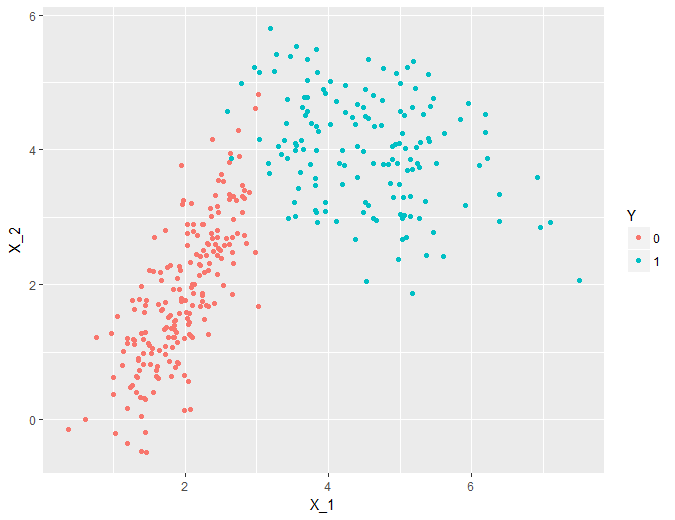
\includegraphics[width = .9\textwidth]{Tests/Test1/GroupPlot}
  \caption{\textbf{Primer ejemplo}. Poco traslape entre puntos}
 \label{fig:Test1Plot}
\end{figure}
Los parámetros se escogieron con un proceso de \textit{prueba y error} para dar estructura pero a la vez separación en el espacio de covariables $\mathcal{X}^2 \approx [0.3,7.5]\times[-0.5,5.9]$. Esto, para que se tuviera una pequeña región donde las distribuciones se traslaparan y exista cierto grado de confusión. El objetivo del modelo, es poder hacer una separación de estas dos regiones sin sobreajustar; identificando, a grandes rasgos, dónde se encuentran los puntos rojos y dónde se encuentran los puntos azules.\\

\subsubsection*{Modelo probit frecuentista para comparar}
En un modelo tradicional, solo se puede hacer una separación lineal. Para comparar, se corrió el siguiente modelo probit frecuentista en \verb|R|, usando la función \verb|glm(..., family = binomial(link = 'probit'))|:
\begin{align}
	p_i & = P(y_i = 1) =\E[y|\xni] = \Phi(f(\xni))  \quad \Rightarrow  			\nonumber \\
	\Phi^{-1}(p_i) &= \beta_0 + \beta_1x_{i,1} + \beta_2x_{i,2} 
	\qquad 	\forall i =1,\ldots,n \label{ec:Test1ModGLM}
\end{align}
De donde se obtuvieron los siguientes resultados:
\begin{align*}
\begin{array}{c|c}
\text{Parámetro} &\text{Valor Estimado} \\
\hdashline
\hat{\beta_0} & -17.29 \\
\hat{\beta_1} & 4.43 \\
\hat{\beta_2} & 1.08 \\
\hline
\text{Métricas} & \text{Valor} \\
\hdashline
ll & 0.0399
\end{array}
\qquad\qquad\qquad
\matconf{198}{2}{200}{2}{148}{150}{200}{150}{350}
\end{align*}
Dada la simplicidad de los datos, el modelo lineal probit, presentado en la ecuación (\ref{ec:Test1ModGLM}) resulta ser una excelente forma de hacer la clasificación. Como se ve en la Figura: \ref{fig:Test1ModGLM}, los datos son fácilmente separables por una linea recta que cruza exactamente donde se empiezan a traslapar. Únicamente, existen 4 datos que quedan mal clasificados, pero que, dadas sus coordenadas, parecerían pertenecer a los grupos opuestos y se consideran como datos atípicos. El modelo presenta una precisión de $98.85\%$, todos los parámetros fueron significativos\footnote{Usando las pruebas $t$ clásicas de modelos lineales frequentistas.} y se tiene un valor de la función log-loss muy bajo. Por lo tanto, se puede concluir que el modelo probit tradicional, es un muy buen modelo para este conjunto de datos. 
\begin{figure}[h]
  \centering
      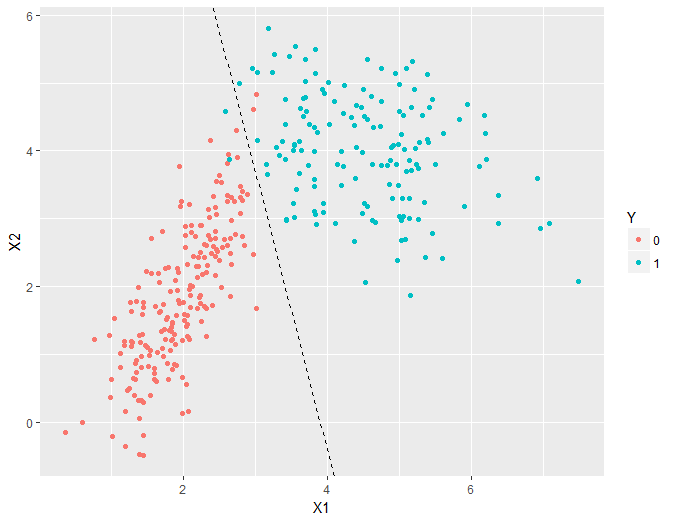
\includegraphics[width = .5\textwidth]{Tests/Test1/GLM_Line}
  \caption{Separación de los grupos por medio de un modelo probit lineal frecuentista}
 \label{fig:Test1ModGLM}
\end{figure}

\subsubsection*{Primer ejemplo del modelo bpwpm}
Ahora, se prueba contra el modelo \textit{bpwpm} de este trabajo. Se esperaría que, al menos, se comportara como el probit anterior, pues, dada la estructura tan robusta que se tiene, este podría colapsar en uno lineal. \\

Como un primer ejemplo sencillo de comprender, se corren un modelo donde los polinomios por partes son rectas disjuntas en cada segmento con un solo nodo. Se realizan mil simulaciones del muestreo Gibbs, de donde se descartan las primeras 500 observaciones y posteriormente se toma cada segunda observación. Estas especificaciones se resumen en la siguiente tabla que se presentará antes de cada modelo. \\
$$\paramsmod{2}{2}{0}{4}{2}{350}{1000}{500}{2}$$
Dado que este es un modelo extremadamente sencillo y que se tiene un número pequeño de bases para los polinomios, $\N = 4$, se presenta por única ocasión, la expansión completa para poderla comparar contra el modelo anterior (\ref{ec:Test1ModGLM}). Esto es\footnote{Para $w_{l,j}$, se usa la convención de subíndices $l = \for{1}{\N}$ de la biyección de la Tabla \ref{tab:Biyeccion} y $j = \for{1},{d}$ para indicar la dimensión}: 
\begin{align}
	p_i &= P(y_i = 1) =\E[y|\xni] = \Phi(f(\xni))  \quad \Rightarrow  			\nonumber \\
	\Phi^{-1}(p_i) = \;&\beta_0 + \beta_1f_1(x_{i,1}) + \beta_2f_2(x_{i,2}) 
	\qquad 	\forall i = \for{1,n}\label{ec:Test1Ej1} \\
	&= \beta_0 \nonumber \\
	&+ \beta_1[w_{1,1} + w_{2,1}x_{i,1} + w_{3,1} + w_{4,1}(x_{i,1} - \t_{1,1})_+] \label{ec:Test1Ej1F1}\\
	& +\beta_2[w_{1,2} + w_{2,2}x_{i,2} + w_{3,2} + w_{4,2}(x_{i,2} - \t_{1,2})_+] \label{ec:Test1Ej1F2}
\end{align}
Contrastando (\ref{ec:Test1ModGLM}) contra (\ref{ec:Test1Ej1}), se puede ver la introducción del componente no lineal a través de las $f_j$, desglosadas en (\ref{ec:Test1Ej1F1}) y (\ref{ec:Test1Ej1F2}), para un total de 11 parámetros. Las expansiones truncadas de polinomios son relativamente sencillas y se ve claramente que se les da estructura de recta, permitiendo discontinuidades entre ellas pues $(\cdot)_+$ es una función por partes que se activa si $x_{i,j}$ es mayor que el nodo $\tau{\cdot,j}$. Aunque esta expansión es aparatosa, el modelo logra hacer excelentes predicciones en cuanto a las regiones. Cabe mencionar que, dado este es un ejemplo introductorio con un número relativamente bajo de observaciones, la estimación de los parámetros, se realizó \textit{dentro de la muestra}\footnote{\textit{in-sample}}, esto quiere decir, que el modelo se entrena con las mismas observaciones contra las que se busca predecir\footnote{El efecto que esto podría tener es que se sobreajuste o se hagan predicciones demasiado acertadas, sin embargo, es normal hacerlo para este tipo de modelos dado $n$. Además, por lo pronto el objetivo final es dar predicciones a través de las regiones formadas y no tanto para observaciones nuevas. De cualquier forma, se podría hacer separando, antes del análisis, la base de datos en dos, una para entrenar el modelo y otra para probarlo.}. Previo al análisis de convergencia de las cadenas, se hace una exploración preliminar para explicar todos los detalles del modelo. Usando la función de perdida cuadrática, se obtienen los siguientes resultados:
\begin{align*}
\resultados{\text{Media posterior}}{98.85}{0.03702}
\quad\quad
\begin{array}{c|c}
\multicolumn{2}{c}{\hat{\beta}} \\
\hline
\hat{\beta_0} & -0.79 \\
\hat{\beta_1} & 3.35 \\
\hat{\beta_2} & 0.65 \\
\end{array}
\quad\quad
\begin{array}{c|c}
\multicolumn{2}{c}{\hat{\wsn}} \\
\hline
-0.52 	& -1.48 \\
0.39	& -0.38 \\
0.09	& 0.66 \\
1.05	& 1.32
\end{array}
\quad\quad
\matconf{198}{2}{200}{2}{148}{150}{200}{150}{350}
\end{align*} 
Numéricamente, el modelo se ve bien; la matriz de confusión es idéntica a la del probit anterior y, por ende, la precisión. Sin embargo, se tiene un valor de la función log-loss un poco más bajo, indicando que se tiene un mejor modelo una vez consideradas las probabilidades ajustadas $\hat{\psn}$. Sin embargo, a diferencia del modelo anterior, los parámetros estimados $\hat{\beta}$ y $\hat{\wsn}$ no se pueden interpretar de la misma manera. En modelos de ML, debido a la complejidad, es mejor tratar a los parámetros como partes funcionales del modelo, que como números con significado. Sin embargo en especial el vector $\hat{\beta}$ puede considerarse como los \textit{pesos} que se le dan a cada transformación no lineal, y su magnitud corresponde a que tanta fuerza tiene esa dimensión en el modelo. De este ejemplo se ve claramente que la primer dimensión, es con la que mejor se están explicando los datos.\\

La Figura \ref{fig:Test1Ej1}, es clave para entender el modelo, en ella se presentan las dos regiones (de colores) que el modelo detecta para hacer las predicciones.
\begin{figure}[h]
	\centering
	\begin{subfigure}[b]{0.45\textwidth}
    	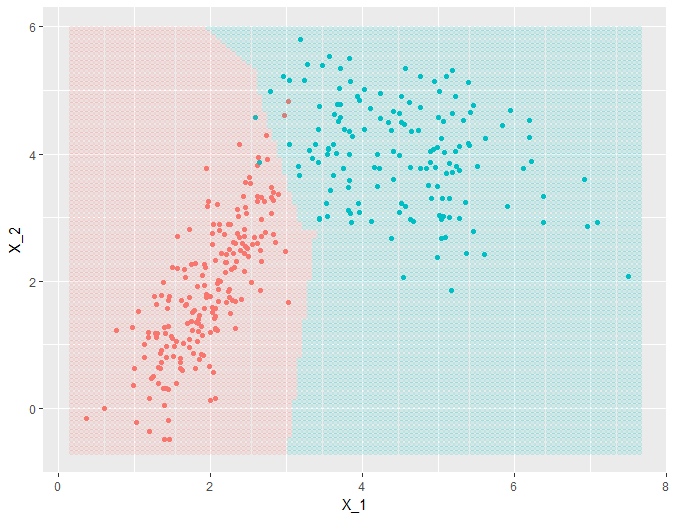
\includegraphics[width =\textwidth]{Tests/Test1/Ej1}
		\caption{Regiones de predicción para modelo con $M = 2$, $J = 2$ y $K = 0$}
	\label{fig:Test1Ej1}
	\end{subfigure}
	\hfill    
    \begin{subfigure}[b]{0.45\textwidth}
        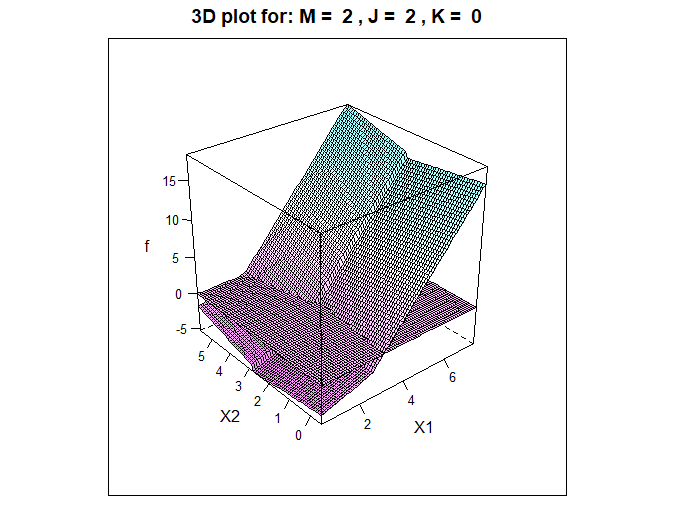
\includegraphics[width=\textwidth]{Tests/Test1/3D}
        \caption{Representación en 3D de $\hat{f}$}
        \label{fig:Test1Ej13D}
    \end{subfigure}
    \caption{Visualización de los resultados del modelo}
\end{figure}
A diferencia de los modelos lineales donde la frontera de predicción binaria es, por ende, lineal, el modelo presentado en este trabajo permite tener fronteras tan complejas como se quiera (aunque no siempre necesarias). Para este ejemplo en particular, la frontera refleja que se está usando un solo nodo y polinomios lineales discontinuos, es por ello que se da la rugosidad. Encontrar la frontera como tal, resulta una tarea mucho más complicada, pues correspondería a resolver la ecuación  $\hat{f}(\xsn) \equiv 0$; en los GLM, esta frontera es perfectamente lineal y el despeje se puede hacer. Sin embargo, cuando se tienen modelos no lineales, se puede hacer una proyección de ella pues, recordando, lo que interesa es discernir cuando la función $\hat{f}$ sea positiva o negativa. Gracias al hecho que $d = 2$ para este ejemplo, se puede visualizar $\hat{f}(\xsn)$ en la Figura \ref{fig:Test1Ej13D}. En esta gráfica, se marca con un plano el \textit{corte} cuando $\hat{f}(\xsn)$ se vuele positiva. Además. se detectan los \textit{pliegues} de discontinuidades derivados del nodo y de la especificación en los parámetros $\MJK$. Se hace notar, que esta representación, no es más que la suma ponderada (por $\hat{\beta})$ de las transformaciones no lineales $f_j \quad j=1,2$, por lo cual vale la pena visualizarlas en la Figura \ref{fig:Test1Ej1Fs}. \\
\begin{figure}[h]
    \begin{subfigure}[b]{0.45\textwidth}
        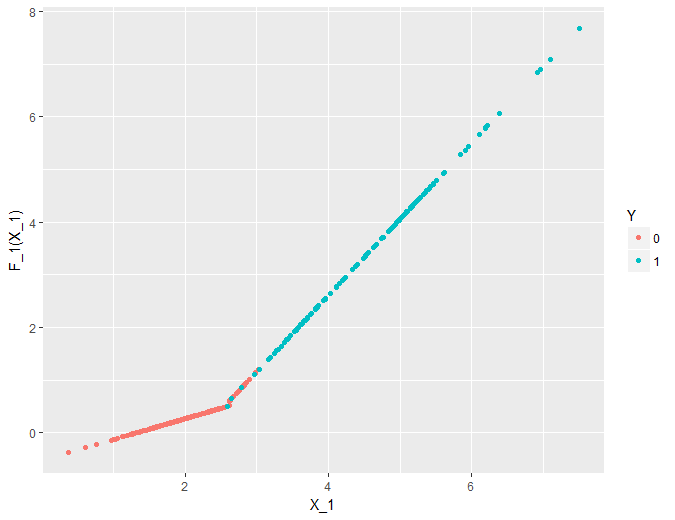
\includegraphics[width=\textwidth]{Tests/Test1/f1}
        \caption{$\hat{f}_1(x_1)$}
    \end{subfigure}
	\hfill
	    \begin{subfigure}[b]{0.45\textwidth}
        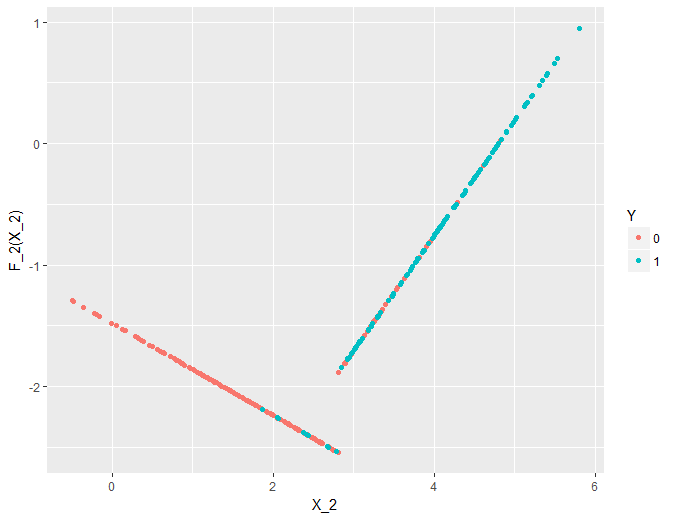
\includegraphics[width=\textwidth]{Tests/Test1/f2}
        \caption{$\hat{f}_2(x_2)$}
    \end{subfigure}
    \caption{Transformaciones no lineales para cada dimensión.}\label{fig:Test1Ej1Fs}
\end{figure}

Aunque la escala vertical de $f_j$ es arbitraria, pues en realidad  están ajustando a los residuales parciales, están cumpliendo su propósito de detectar y capturar el patrón que deriva en la separación de los grupos. Para valores izquierdos de ambas variables, se tiene el grupo rojo, para valores mayores, se tiene el grupo azul. Ese efecto, es capturado en el salto que dan las rectas en el nodo, mediante una mayor pendiente en las rectas del lado derecho (mayoritariamente azules), pues, al ser más positivas conforme se avanza en el rango de $x$, estas tendrán más peso en la función de proyección $\hat{f}$, volviéndola más positiva y por ende, más probable que esa región contenga observaciones del grupo azul.\\

% que ya quede claro todo pues ya se incorporó todo 
Con estas gráficas, se espera dar claridad a todos los componentes del modelo. % Mencionar que muchos elementos son más técnicos que nada como z.
% Mencionar que las interacciones entre los nodos son un pedote

% Mencionar las cadenas de Markov de las primeras imágenes
% Mencionar que dada la estocasticidad los resultados pueden variar, que dada la estructura normal usar entre la media y asi vale verga igual que (usually) los de Thin y asi. 
% Que si las 4 observaciones estuvieran dentro se estaría sobreajustando

\subsection{Análisis de Sensibilidad}
% Moverle el bote y ver que vale verga si se usan polinomios muy pequeños :( como nos gustaría. 
% Que a medida que subimos el número de parámetros, la estabilidad mejora chingos. 

\subsection{Análisis de Convergencias}
%No quiero llegar aquí


\section{Otros resultados interesantes}
Estos ejemplos, son más expositivos que analíticos, es decir, se analizan más las caracteristicas fundamentales que todos los detalles del modelo como se hizo en la sección anterior. Sin embargo, usando el paquete, se puede hacer el análisis de la misma forma. 
%Dar gráficas y resultados de: la normal modificada, datos parabolicos, circulares y hopefully Ying-Yang.

\section{Prueba con datos reales}
%Hacer prueba con datos SVSS y con dato de Hastie and Tibsh, y los de Ovando, si me los manda el cabrón

\end{document}